% Gemini theme
% See: https://rev.cs.uchicago.edu/k4rtik/gemini-uccs
% A fork of https://github.com/anishathalye/gemini

\documentclass[final]{beamer}

% ====================
% Packages
% ====================

\usepackage[T1]{fontenc}
\usepackage{lmodern}
\usepackage[size=custom,width=120,height=72,scale=1.0]{beamerposter}
\usetheme{gemini}
% \usecolortheme{uchicago}
\usecolortheme{stanford}
\usepackage{graphicx}
\usepackage{booktabs}
\usepackage{tikz}
\usepackage{pgfplots}
\usepackage{adjustbox}
\usepackage[table]{xcolor}
\usepackage{colortbl}
\pgfplotsset{compat=1.17}
% !TeX program = xelatex

% ====================
% Lengths
% ====================

% If you have N columns, choose \sepwidth and \colwidth such that
% (N+1)*\sepwidth + N*\colwidth = \paperwidth
\newlength{\sepwidth}
\newlength{\colwidth}
\setlength{\sepwidth}{0.025\paperwidth}
\setlength{\colwidth}{0.3\paperwidth}

\newcommand{\separatorcolumn}{\begin{column}{\sepwidth}\end{column}}


\title{Preschool children reason about third-party goals when evaluating acoustic environments}


\author{Rondeline M. Williams and Michael C. Frank}

\institute[shortinst]{Department of Psychology, Stanford University\\Stanford, CA 94305 USA}


% ====================
% Footer (optional)
% ====================

\footercontent{
  \href{rylanschaeffer.github.io}{rylanschaeffer.github.io} \hfill
  NeurIPS 2021 Workshop: Metacognition in the Age of AI \hfill
  \href{mailto:rylanschaeffer@gmail.com}{rylanschaeffer@gmail.com}}
% (can be left out to remove footer)

% ====================
% Logo (optional)
% ====================

% use this to include logos on the left and/or right side of the header:
% \logoright{\includegraphics[height=7cm]{logos/cs-logo-maroon.png}}
% \logoleft{\includegraphics[height=7cm]{logos/cs-logo-maroon.png}}

% ====================
% Body
% ====================

\begin{document}

% This adds the Logos on the top left and top right
\addtobeamertemplate{headline}{}
{
    \begin{tikzpicture}[remember picture,overlay]
    %   \node [anchor=north west, inner sep=3cm] at ([xshift=0.0cm,yshift=1.0cm]current page.north west)
    %   {\includegraphics[height=5.0cm]{stanford_logos/Stanford-CS.png}}; % uc-logo-white.eps
      \node [anchor=north east, inner sep=3cm] at ([xshift=0.0cm,yshift=2.5cm]current page.north east)
      {
\includegraphics[height=7.0cm]{stanford_logos/Block_S_2_color.png}};
    \end{tikzpicture}
}

\begin{frame}[t]
\begin{columns}[t]
\separatorcolumn

\begin{column}{\colwidth}

  \begin{block}{Introduction}

    \begin{itemize}
      \item \textbf{Children as flexible learners}
        \begin{itemize}
          \item Learning flexibility in children includes:
            \begin{itemize}
              \item Adjusting attention to stimuli that is learnable (Gerken et al., 2011; Kidd, 2011)
              \item Using emotional expressions as cues for novel object exploration (Wu \& Gweon, 2021)
              \item Reasoning about environmental structure and goals to determine approach strategies (Meder et al., 2021)
            \end{itemize}
        \end{itemize}
      \item \textbf{Background noise and learning}
        \begin{itemize}
          \item Acoustic noise is ubiquitous
          \item Repeated noise exposure influences learning and development in critical ways:
            \begin{itemize}
              \item Reduces speech perception and word recognition (Klatte et al., 2013; Bjorklund et al., 1990)
              \item Decreases word learning (McMillan \& Saffran, 2016)
              \item Impinges on already limited cognitive resources for adaptive strategy building (Loh et al., 2022)
            \end{itemize}
        \end{itemize}
      \item \textbf{(Ecological) Active learning}
        \begin{itemize}
          \item Traditional active learning:
            \begin{itemize}
              \item Learners interact with individual stimuli within their environment (Settles, 2009)
              \item Accurate stimuli labeling is a primary goal
            \end{itemize}
          \item Ecological active learning:
            \begin{itemize} 
              \item Children learn by tracking environmental features and adapt their exploration strategies accordingly (Ruggeri, 2022)
              \item Exploratory strategies for learning are context-dependent 
              \item Exploit statistical regularities in the environment to reduce demands on cognition
            \end{itemize}
        \end{itemize}
      \item \textbf{Environmental selection}
        \begin{itemize}
          \item Learners preferentially select acoustic environments that align with a set of goals
          \item Emphasizes acoustic information
          \item Goal-directed
          \item Addresses variabilities across environments
          \item Children can rely exclusively on acoustic information to make exploration decisions
        \end{itemize}
    \end{itemize}       

    Lorem ipsum dolor sit amet, consectetur adipiscing elit. Morbi ultricies
    eget libero ac ullamcorper. Integer et euismod ante. Aenean vestibulum
    lobortis augue, ut lobortis turpis rhoncus sed. Proin feugiat nibh a
    lacinia dignissim. Proin scelerisque, risus eget tempor fermentum, ex
    turpis condimentum urna, quis malesuada sapien arcu eu purus.

  \end{block}

  \begin{block}{Background: Metacognition}

    Nam vulputate nunc felis, non condimentum lacus porta ultrices. Nullam sed
    sagittis metus. Etiam consectetur gravida urna quis suscipit.

    \begin{itemize}
      \item \textbf{Mauris tempor} risus nulla, sed ornare
      \item \textbf{Libero tincidunt} a duis congue vitae
      \item \textbf{Dui ac pretium} morbi justo neque, ullamcorper
    \end{itemize}

    Eget augue porta, bibendum venenatis tortor.

  \end{block}
  
    \begin{block}{Research question}
    
    \end{block}

  \begin{alertblock}{A highlighted block}

    To what extent do preschool children use environmental selection as an adaptive strategy for learning in noisy acoustic environments?

  \end{alertblock}

\end{column}

\separatorcolumn

\begin{column}{\colwidth}

  \begin{block}{Methods}

    \begin{itemize}
      \begin{table}[ht]
        \centering
        \begin{tabular}{|p{0.3\linewidth}|p{0.15\linewidth}|p{0.15\linewidth}| p{0.15\linewidth}|}
          \hline
          \right
          \rowcolor{cardinalred!80}
          \multicolumn{2}{|c|}{\textbf{Experiment 1}} & \multicolumn{2}{c|}{\textbf{Experiment 2}} \\
          \cline{2-4}
          \rowcolor{cardinalred!80}
          \multicolumn{1}{|c|}{\textbf{}} &
          \multicolumn{1}{|c|}{\textbf{Children}} & 
          \multicolumn{1}{|c|}{\textbf{Children}} & 
          \multicolumn{1}{|c|}{\textbf{Adults}} \\
          \hline
          N & 72 & 54 & 37 \\
          \hline
          \rowcolor{cardinalred!40}
          $\mu$ & 4.46 years & 4.55 years & 40.43 years \\
          \hline
          \raggedright African American/Black & 4.2\% & 3.7\% & 4.2\% \\ 
          \hline
          \rowcolor{cardinalred!40}
          \raggedright Asian American/Pacific Islander & 23.6\% & 37\% & x\% \\
          \hline
          Caucasian/White & 27.8\% & 31.5\% & 70.3\% \\
          \hline
          \rowcolor{cardinalred!40}
          Multiracial & 26.4\% & 20.4\% & x \\
          \hline
          Hispanic/Latinx & 8.3\% & 7.4\% & x \\
          \hline
          \rowcolor{cardinalred!40}
          Other & 8.3\% & & \\
          \hline
        \end{tabular}
      \end{table}         
    
    \end{itemize} 

    \begin{itemize}
      \item \textbf{Experiment 1}
    \end{itemize}
    \begin{figure}
      \begin{minipage}[t]{0.2\linewidth}
        \centering
        
\includegraphics[width=2in, height=2in]{figures/dance.png}
        \caption{Dance}
      \end{minipage}
      \begin{minipage}[t]{0.2\linewidth}
        \centering
        
\includegraphics[width=2in, height=2in]{figures/read.png}
        \caption{Read}
      \end{minipage}%
      \begin{minipage}[t]{0.2\linewidth}
        \centering
        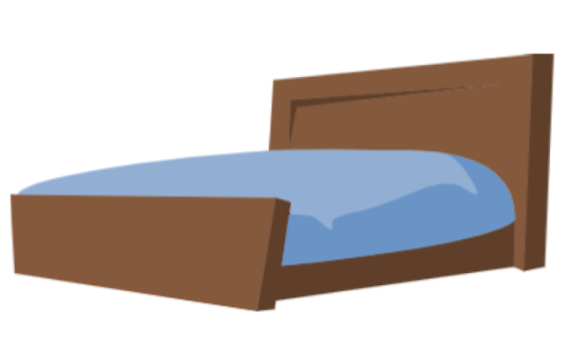
\includegraphics[width=2in, height=2in]{figures/sleep.png}
        \caption{Sleep}
      \end{minipage}
      \begin{minipage}[t]{0.2\linewidth}
        \centering
        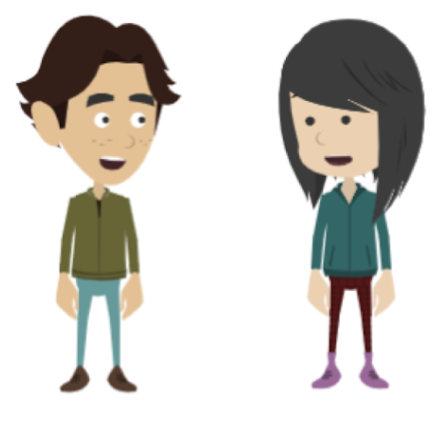
\includegraphics[width=2in, height=2in]{figures/talk.png}
        \caption{Talk}
      \end{minipage}
    \end{figure}    

    \begin{itemize}
      \item \textbf{Experiment 2}
    \end{itemize}
    \begin{figure}
      \begin{minipage}[t]{0.2\linewidth}
        \centering
        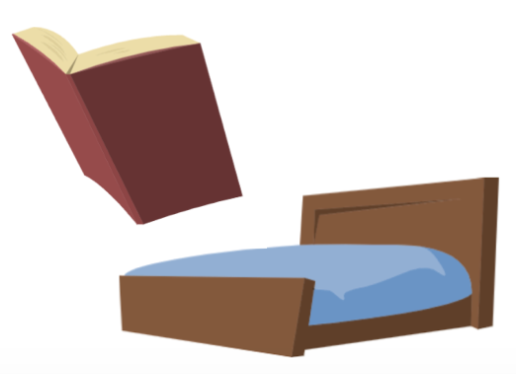
\includegraphics[width=2in, height=2in]{figures/fraw.png}
        \caption{Dance}
      \end{minipage}
      \begin{minipage}[t]{0.2\linewidth}
        \centering
        
\includegraphics[width=2in, height=2in]{figures/gobb.png}
        \caption{Read}
      \end{minipage}%
      \begin{minipage}[t]{0.2\linewidth}
        \centering
        
\includegraphics[width=2in, height=2in]{figures/plip.png}
        \caption{Sleep}
      \end{minipage}
      \begin{minipage}[t]{0.2\linewidth}
        \centering
        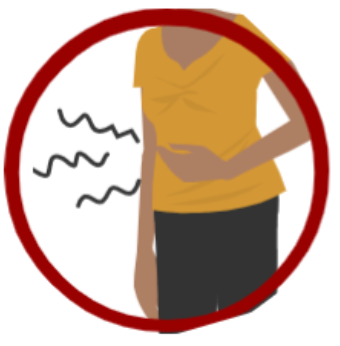
\includegraphics[width=2in, height=2in]{figures/terb.png}
        \caption{Talk}
      \end{minipage}
    \end{figure}
    
    \begin{figure}
      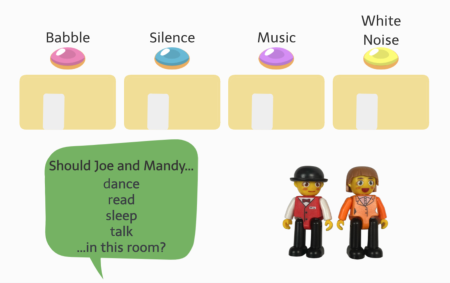
\includegraphics[width = 14in, height = 7in]{../writeup/figs/e3-stimuli-1.pdf}
    \end{figure}
  
  \end{block}

\end{column}

\separatorcolumn

\begin{column}{\colwidth}

  \begin{block}{Results}

    \begin{figure}
      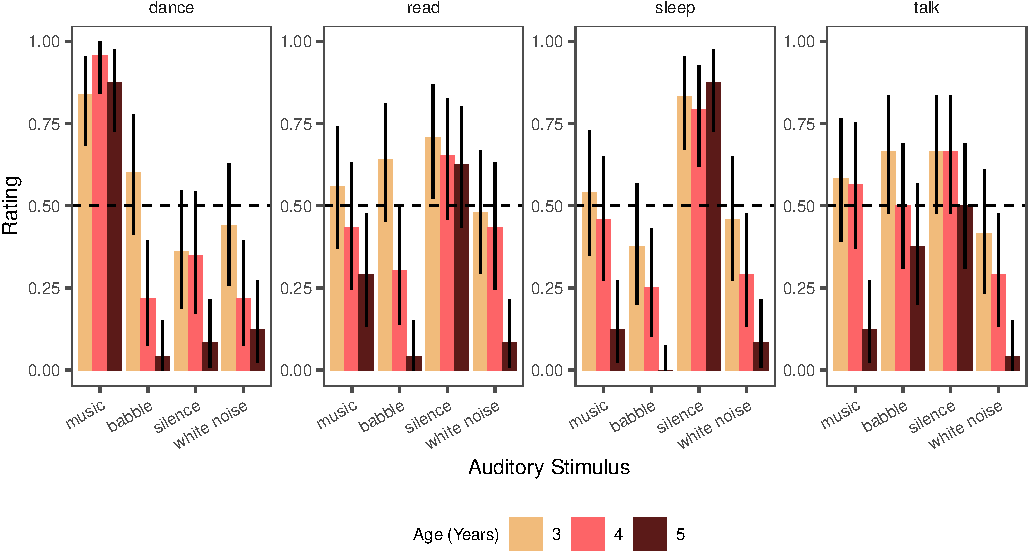
\includegraphics[width = 14in, height = 7in]{../writeup/figs/e3b-bar-1.pdf}
    \end{figure}

    \begin{figure}
      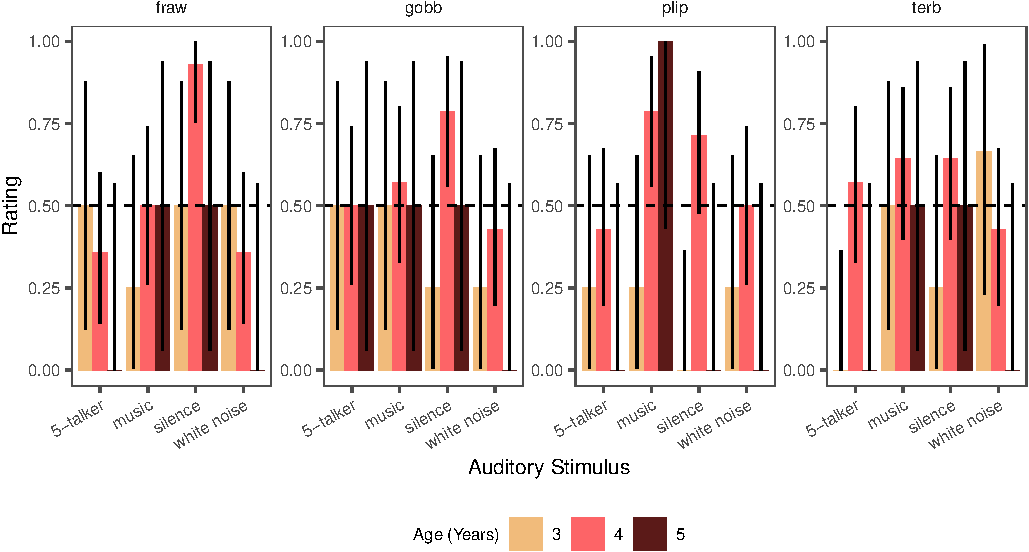
\includegraphics[width = 14in, height = 7in]{../writeup/figs/e4b-bar-1.pdf}
    \end{figure}

    \heading{A heading inside a block}

    Praesent consectetur mi $x^2 + y^2$ metus, nec vestibulum justo viverra
    nec. Proin eget nulla pretium, egestas magna aliquam, mollis neque. Vivamus
    dictum $\mathbf{u}^\intercal\mathbf{v}$ sagittis odio, vel porta erat
    congue sed. Maecenas ut dolor quis arcu auctor porttitor.

    \heading{Another heading inside a block}

    Sed augue erat, scelerisque a purus ultricies, placerat porttitor neque.
    Donec $P(y \mid x)$ fermentum consectetur $\nabla_x P(y \mid x)$ sapien
    sagittis egestas. Duis eget leo euismod nunc viverra imperdiet nec id
    justo.

  \end{block}

  \begin{block}{Nullam vel erat at velit convallis laoreet}

    Class aptent taciti sociosqu ad litora torquent per conubia nostra, per
    inceptos himenaeos. Phasellus libero enim, gravida sed erat sit amet,
    scelerisque congue diam. Fusce dapibus dui ut augue pulvinar iaculis.

  \end{block}

  \begin{block}{References}

    \nocite{*}
    \footnotesize{\bibliographystyle{plain}\bibliography{poster}}

  \end{block}

\end{column}

\separatorcolumn
\end{columns}
\end{frame}

\end{document}
